\subsection{Datenbankentwurf}
\label{sec:Datenbankentwurf}

Aufbauend auf den vorangegangenen Entwurfsergebnissen wird im Folgenden ein Entwurf der Datenbank angefertigt. Dieser Entwurf benutzt zur grafischen Modellierung ein Tabellenmodell\footnotemark.

\footnotetext{Ein Tabellenmodell ist ein graphisches Modell zur Darstellung der inneren Datenbankstruktur einer Datenbank. In diesem Modell werden Tabellen, deren Attribute (Eigenschaften) und die Beziehung zu anderen Tabellen dargestellt.}

Bevor das Tabellenmodell erstellt werden kann müssen aus dem vorliegenden Projekt die Bestandteile identifiziert werden, die persistent in der Datenbank gespeichert werden müssen.
Aus dem vorgangenen Oberflächenentwurf wird deutlich, dass das Projekt Inhaltich aus zwei Teilen besteht, einer Benutzeransicht und einer Administrationsansicht. Die Benutzeransicht stellt dabei nur Informationen dar, die in der Administrationsansicht gepflegt und hinterlegt wurden. Der Administrationsbereich ist der datenhaltende Bereich, in dem die Interaktion mit der Datenbank stattfindet. In dem \verweis{Administrationsbereich} werden dabei bereits 3 Informationsobjekte deutlich:

\begin{itemize}
  \item Infotexte
  \item Fotos
  \item Administratordaten
\end{itemize}

Die Beziehung zwischen Infotexten und Fotos stellt dabei eine sogenannte n:m (gesprochen: n zu m) Beziehung dar, das bedeutet ein Infotext kann mehreren Fotos zugeordnet sein und im Gegenzug könnnen ebenso mehrere Infotexte auf demselben Foto platziert werden. In einem solchen Fall muss eine neue Tabelle angelegt werden, in der die Beziehung zwischen Foto und Infotext gespeichert wird. Gleiches gilt für die Nachbarschaftsbeziehung zwischen zwei Fotos. Da ein Foto theoretisch unendlich viele Nachbarfotos haben kann braucht es wiederrum eine weitere Tabelle für die Beziehung zwischen Foto und Nachbarfoto. Neben diesen zwei zusätzlichen Tabellen braucht es noch drei weitere für die Darstellung der Übersichtskarte. In der Übersichtskarte soll grundsätzlich zwischen dem Studienstandort an der Baccumerstraße und dem Standort an der Kaiserstraße unterschieden werden. Da beide Standorte unterschiedlich parametresiert werden braucht es hierfür eine erste eigene Tabelle (diese wird im Folgenden mit dem Namen \textit{area} bezeichnet). Diese areas beschreiben einen topologischen Auschnitt einer Google Maps\copyright\ Karte. Da eine topologische Karte nur den Umriss von Gebäuden zeigt, ist es schwer den genauen Standort eines Panoramas zu bestimmen. Aus diesem Grund werden Vektorgrafiken über die Karte gelegt, die das "`Innenleben"'(Wände, Gebäudetrackte, etc.) des Campus zeigen. Sowohl die topologische Karte als auch die übergelegten Grafiken (im folgenden \textit{overlays} genannt) brauchen eine eigene Tabelle, da beide jeweils noch weitere Attribute haben. Ein Overlay ist dabei immer einer Karte zugeordnet, eine Karte kann aber mehrere Overlays besitzen. Über die Zuordnung von mehreren Overlays zu einer Karte werden Stockwerke an einem Standort dargestellt. Ein Overlay enthält damit unter anderem den Pfad zu einer Grafik, die ein Stockwerk an einem Standort repräsentiert. Zusamengefasst ergeben sich damit folgende Tabellen:

\begin{itemize}
  \item Infotext (Verwaltung der Infotexte)
  \item Panorama (Verwaltung der Fotos)
  \item admin (Verwaltung der Administratordaten)
  \item Infotext\_panorama (n:m Beziehung zwischen Infotexten und Fotos)
  \item neighbour (n:m Nachbarschaftsbeziehung zwischen zwei Fotos)
  \item area (Kartenbereich)
  \item map (Kartenansicht)
  \item overlay (übergelegte Grafik)
\end{itemize}

Diese Tabellen werden in folgendem Tabellenmodell mit ihren jeweiligen Attributen dargestellt.

\begin{figure}[htb]
\centering
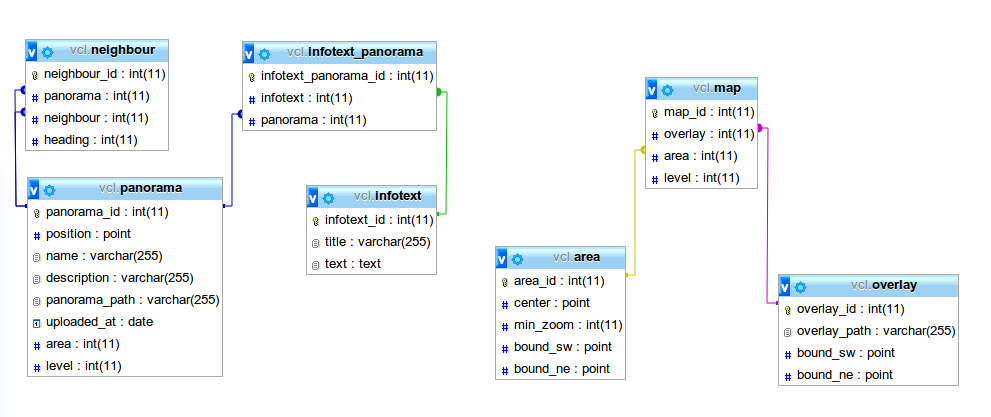
\includegraphics[width=1.0\textwidth]{Tabellenmodell.png}
\caption[Tabellenmodell der Anwendung]{Tabellenmodell der Anwendung\protect\footnotemark}
\label{fig:Tabellenmodell}
\end{figure}
\footnotetext{Quelle: Eigene Darstellung}